\RequirePackage[l2tabu, orthodox]{nag}
\documentclass[12pt]{article}
\usepackage[utf8]{inputenc} 
\usepackage[T1]{fontenc}
\usepackage[english]{babel} 
\usepackage[margin=2.5cm]{geometry}
\geometry{a4paper}
\usepackage{longtable}


%----------------------------KODE START---------------------------------------
\usepackage{listings}
\usepackage{color}
\usepackage[usenames,dvipsnames]{xcolor}
\definecolor{gray}{rgb}{0.5,0.5,0.5}
\definecolor{mauve}{rgb}{0.58,0,0.82}
\lstset{
  basicstyle=\footnotesize,
  numbers=left,
  numberstyle=\tiny\color{gray},
  stepnumber=1,
  numbersep=10pt,
  backgroundcolor=\color{white},
  showspaces=false,               % show spaces adding particular underscores
  showstringspaces=false,         % underline spaces within strings
  showtabs=false,                 % show tabs within strings adding particular underscores
  frame=single,                   % adds a frame around the code
  rulecolor=\color{black},        
  tabsize=4,
  captionpos=b,                   % sets the caption-position to bottom
  breaklines=true,                % sets automatic line breaking
  breakatwhitespace=false,        % sets if automatic breaks should only happen at whitespace
  title=\lstname,                   % show the filename of files included with \lstinputlisting;
                                  % also try caption instead of title
  keywordstyle=\color{mauve},          % keyword style
  commentstyle=\color{Maroon},       % comment style
  stringstyle=\color{BlueViolet},         % string literal style
  escapeinside={\%*}{*)},            % if you want to add LaTeX within your code
  morekeywords={*,...},              % if you want to add more keywords to the set
  deletekeywords={...}              % if you want to delete keywords from the given language
}
%----------------------------KODE SLUT----------------------------------------


\setlength\parindent{0pt} % Makes \noindent standard
\usepackage{graphicx} 
\usepackage{sidecap}
\usepackage{caption}
\usepackage{subcaption}
\usepackage{float} 
\usepackage{wrapfig} % Allows in-line images if needed
\usepackage{hyperref}
\usepackage{amsmath}
\usepackage{amsfonts}
\usepackage{mathtools}
\hypersetup{colorlinks=false,hidelinks, citecolor=black, urlcolor=black}
\usepackage{csquotes}
\usepackage{comment}

\usepackage[dot, autosize, outputdir="dotgraphs/"]{dot2texi}
\usepackage{tikz}
\usetikzlibrary{shapes}
\usepackage{url}
\usepackage{booktabs}
\usepackage{multirow}
\usepackage{longtable}
\setcounter{secnumdepth}{4}
\setcounter{tocdepth}{4}
\usepackage[titletoc]{appendix} % Names appendices "Appendix A"
                                % instead of just A in Contents
\usepackage[bottom]{footmisc}
\usepackage{pdfpages}
\usepackage{algorithm}% http://ctan.org/pkg/algorithms
\usepackage{algpseudocode}% http://ctan.org/pkg/algorithmicx


%\usepackage{lmodern}
\usetikzlibrary{arrows,automata}
\usepackage{verbatim}

\linespread{1.2} 
\graphicspath{{./figures/}} 

% fancy drawings
\usepackage{pgf}
\usepackage{epigraph}

% \epigraphsize{\small}% Default
\setlength\epigraphwidth{8cm}
\setlength\epigraphrule{0pt}

\usepackage{etoolbox}

\makeatletter
\patchcmd{\epigraph}{\@epitext{#1}}{\itshape\@epitext{#1}}{}{}
\makeatother

%\usepackage{boxproof}
%\usepackage{nomencl}
\usepackage{natbib}

\newcommand{\fasto}{\textsc{Fasto} }
\newcommand{\mips}{\textsc{Mips} }
\newcommand{\mars}{Mars }
\makeatletter
\def\BState{\State\hskip-\ALG@thistlm}
\makeatother

%-----------------------------------------------------------------------------
\begin{document}
\begin{titlepage}

\centering 

\textsc{\Large \LaTeX{} workshop}\\[0.5cm] 
\textsc{\large Små opgaver, til at få dig i gang}\\[0.5cm] 

\vfill

\emph{Authors:}
\\
Datalogisk \textsc{Fagråd} 
\vspace{20mm}

{\large 01-10-2014}\\[3cm] 

\end{titlepage}
%-----------------------------------------------------------------------------

\tableofcontents
\newpage

%-----------------------------------------------------------------------------

Ideen med disse opgaver er, at gøre dig fortrolig med \LaTeX{}. De er udarbejdet for at give dig et lille indblik i, hvad du kan, og for at give dig nogle små konkrete eksempler, du selv ender med, at have lavet. Man lærer nemlig bedst ved, at prøve selv - ikke ved, at få en skabelon fra andre. \\

Så hyg dig med det, brug Google og menneskerne omkring dig, hvis du ikke på forhånd ved, hvordan du skal løse opgaverne. \\

Det kan anbefales, at bygge din preamble op med kommentarer, sådan at du ved, hvad de forskellige pakker gør og bruges til $\ddot\smile$ . En kommentar i \LaTeX{} laves ved hjælp af \% - sæt tegnet foran en sætning, og vupti - du har en kommentar, som ikke vises i den generede PDF. 

\section{Matematik}
	\begin{enumerate}
  		\item Hvilke pakker, skal bruges for at løse de efterfølgende opgaver?
  		\item Indskriv følgende:
			\begin{enumerate}				
				\item $\frac{1}{2} \cdot \sqrt{5}$
				\item $\forall x \in X, \quad \exists y \leq \epsilon$
				\item $(p \rightarrow q) \wedge (p \rightarrow r) \vdash p \rightarrow q \wedge r$
				\item $\cos (2\theta) = \cos^2 \theta - \sin^2 \theta$
				\item $k_{n+1} = n^2 + k_n^2 - k_{n-1}$
			\end{enumerate}
 		\item Indskriv følgende 2:
\begin{center}
	$A_{m,n} =
 	\begin{bmatrix}
  		a_{1,1} & a_{1,2} & \cdots & a_{1,n} \\
  		a_{2,1} & a_{2,2} & \cdots & a_{2,n} \\
  		\vdots  & \vdots  & \ddots & \vdots  \\
  		a_{m,1} & a_{m,2} & \cdots & a_{m,n}
 	\end{bmatrix}$
\end{center}

\begin{align}
\left(\!
    \begin{array}{c}
      n \\
      r
    \end{array}
  \!\right) = \frac{n!}{r!(n-r)!}
\end{align}
		\item Er der forskel på at skrive $^*$ eller ingen ting efter align i begin\{align\}?
	\end{enumerate}

Alle opgaver burde kunne løses med informationer fra denne side:\\
\url{http://en.wikibooks.org/wiki/LaTeX/Mathematics}

\section{Tabeller}
	\begin{enumerate}
  		\item Hvilke pakker, skal bruges for at løse de efterfølgende opgaver?
  		\item Indskriv følgende tabel i \LaTeX{}:
\begin{table}[H]
\center
\begin{tabular}{c| c| c c c c| c c c}
DFA & NFA & \multicolumn{7}{c}{Transitions} \\
state & states & \texttt{id} & * & = & \$ & S & L & R \\
\hline
0 & A, D, H, J, M, O 	& s4 	& s5 	&     	&      	& g1 	& g2 	& g3\\
1 & B                       	&      &      	&     	& s6 	&      	&      	& \\
2 & E, P                   	&      &     	& s7 	&      	&     	&      	& \\
3 & I                         	&     	&    	&      	&      	&     	&      	& \\
4 & N                       	& 	&     	&      	&      	&     	&      	& \\
5 & K, O, J, M		& 	& s5	& 	& 	& 	& g9	& g8\\
6 & C			& 	& 	&	&	&	&	& \\
7 & F			&	&	&	&	&	&	& g10\\
8 & L				& 	& 	&	&	&	&	& \\
9 & P			& 	& 	&	&	&	&	& \\
10 & G 			& 	& 	&	&	&	&	& \\
\end{tabular}
\end{table}

 		\item Hvad betyder det for ens tabel, hvis man skriver [H] efter begin\{table\}?
	\end{enumerate}

Alle opgaver burde kunne løses med informationer fra denne side:\\
\url{http://en.wikibooks.org/wiki/LaTeX/Tables}

\newpage
\section{Billeder}
	\begin{enumerate}
  		\item Hvilke pakker, skal bruges for at løse de efterfølgende opgaver?
		\item Find et par billeder og placer dem på følgende måder:\\
	
		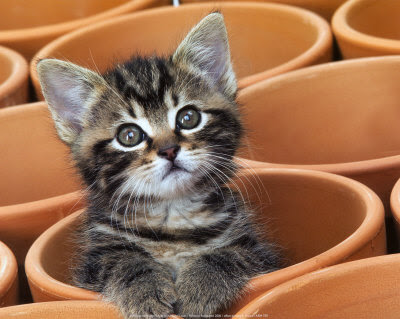
\includegraphics[scale=0.5]{cat}
	
		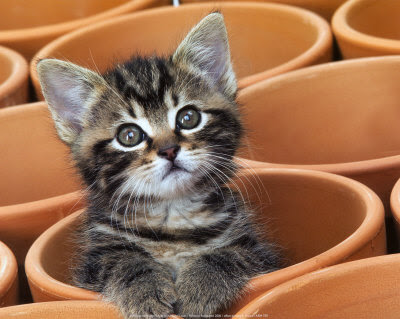
\includegraphics[scale=0.5, angle=180]{cat}
		
		\item Hvordan placerer man to billeder ved siden af hinanden i \LaTeX{}?
		\item Kan man også importere PDF'er til sin fil? I så fald hvordan?
	\end{enumerate}

\newpage
\section{Grafer og andet sjov}
Der er delte meninger om TikZ, men da personen, der har udarbejdet disse opgaver synes, det er et fantastisk værktøj, er her en opgave, der involverer TikZ $\ddot\smile$ - ligesom i opgaverne oven for, går det ud på at genskabe figurerne:\\

\begin{center}
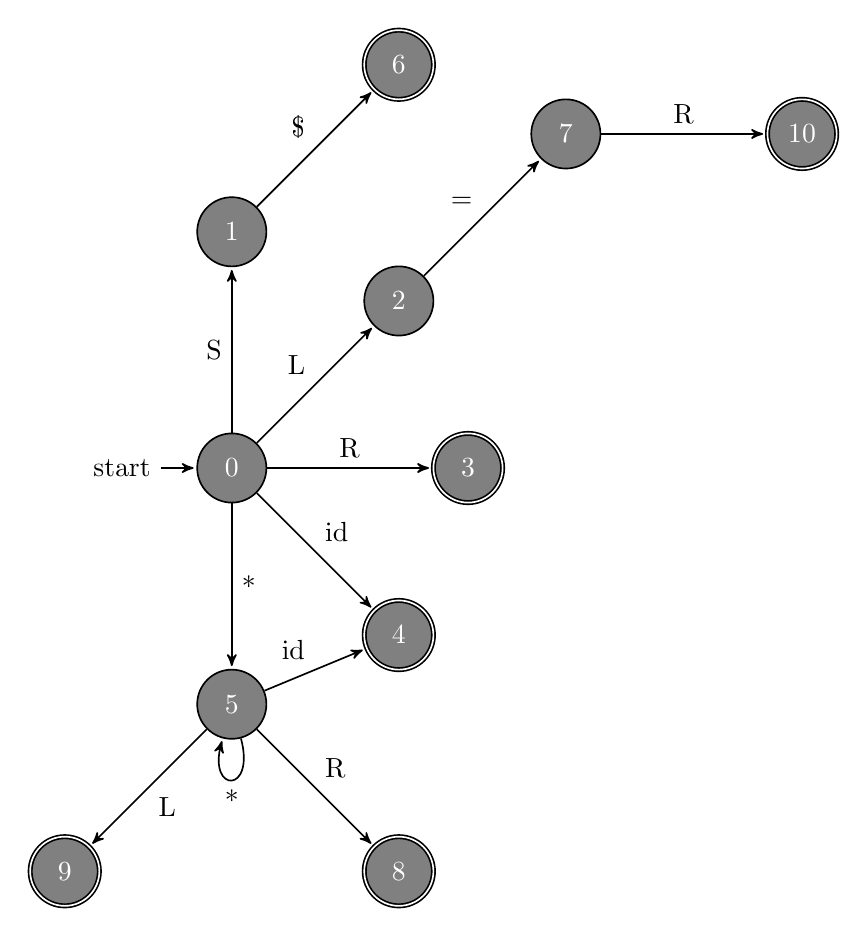
\begin{tikzpicture}[->,>=stealth',shorten >=1pt,auto,node distance=3cm,
                    semithick]
  \tikzstyle{every state}=[fill=gray,text=white]

  \node[initial,state] (0) {$0$};
  \node[state] (1) [above of=0] {$1$};
  \node[state] (2) [above right of=0] {$2$};
  \node[accepting,state] (3) [right of=0] {$3$};
  \node[accepting,state] (4) [below right of=0] {$4$};
  \node[state] (5) [below of=0] {$5$};
  \node[accepting,state] (6) [above right of=1] {$6$};
  \node[state] (7) [above right of=2] {$7$};
  \node[accepting,state] (8) [below right of=5] {$8$};
  \node[accepting,state] (9) [below left of=5] {$9$};
  \node[accepting,state] (10) [right of=7] {$10$};

  
  \path 	(0)	edge node {id} (4)
  			edge node {*} (5)
			edge node {S} (1)
			edge node {L} (2)
			edge node {R} (3)
		(1)	edge node {\$} (6)
		(2)	edge node {=} (7)
		(5)	edge node {id} (4)
			edge [loop below] node {*} (5)
			edge node {R} (8)
			edge node {L} (9)
		(7) 	edge node {R} (10);
                	
\end{tikzpicture}\\
\end{center}

\begin{center}
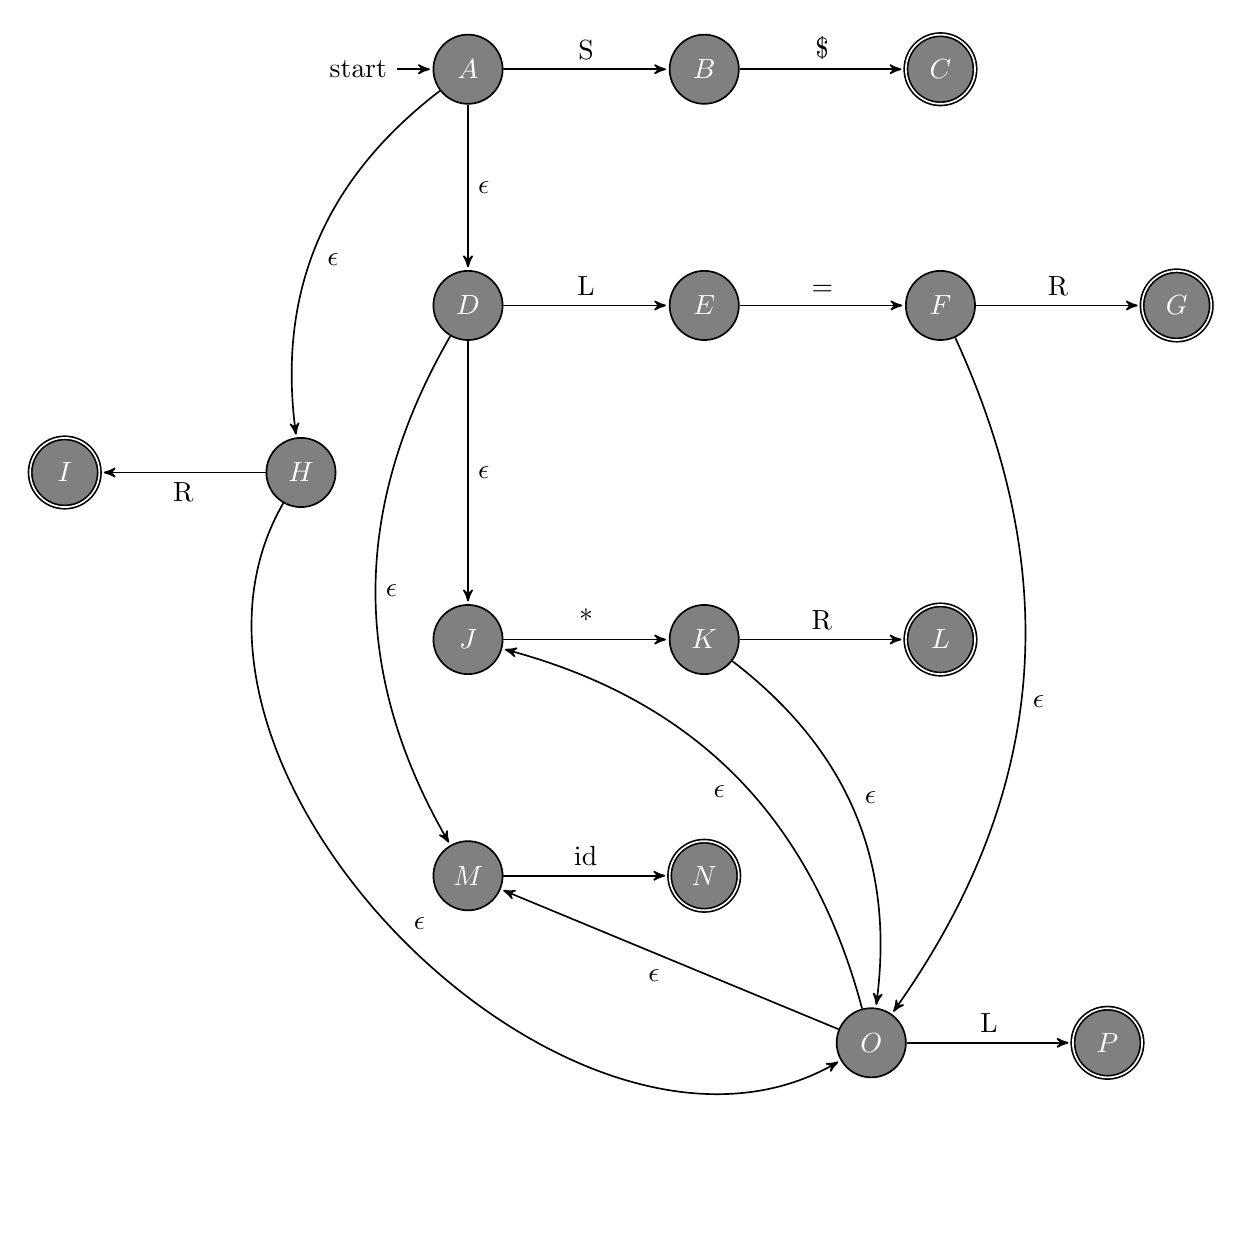
\begin{tikzpicture}[->,>=stealth',shorten >=1pt,auto,node distance=3cm,
                    semithick]
  \tikzstyle{every state}=[fill=gray,text=white]

  \node[initial,state] (A) {$A$};
  \node[state] (B) [right of=A] {$B$};
  \node[accepting,state] (C) [right of=B] {$C$};
  
  \node[state] (D) [below of=A] {$D$};
  \node[state] (E) [right of=D] {$E$};
  \node[state] (F) [right of=E] {$F$};
  \node[accepting,state] (G) [right of=F] {$G$};
  
  \node[state] (H) [below left of=D] {$H$};
  \node[accepting,state] (I) [left of=H] {$I$};
  
  \node[state] (J) [below right of=H] {$J$};
  \node[state] (K) [right of=J] {$K$};
  \node[accepting,state] (L) [right of=K] {$L$};
  
  \node[state] (M) [below of=J] {$M$};
  \node[accepting,state] (N) [right of=M] {$N$};
  
  \node[state] (O) [below right of=N] {$O$};
  \node[accepting,state] (P) [right of=O] {$P$};
  
  \path 	(A)	edge node {S} (B)
                		edge node {$\epsilon$} (D)
                		edge [bend right] node {$\epsilon$} (H)
           	(B)	edge node {\$} (C)
           	(D)	edge node {L} (E)
                 	edge node {$\epsilon$} (J)
                 	edge [bend right] node {$\epsilon$} (M)
           	(E) 	edge node {=} (F)
           	(F) 	edge node {R} (G)
                		edge [bend left] node {$\epsilon$} (O)
		(H)	edge node {R} (I)
			edge [bend right=75] node {$\epsilon$} (O)
		(J)	edge node {*} (K)
		(K)	edge node {R} (L)
			edge [bend left] node {$\epsilon$} (O)
		(M) 	edge node {id} (N)
		(O) 	edge node {L} (P)
		  	edge node {$\epsilon$} (M)
			edge [bend right] node {$\epsilon$} (J);
\end{tikzpicture}\\
\end{center}


\newpage
\section{Keder du dig?}
Hvis du keder dig, så 

\begin{enumerate}
	\item lav et dokument, der ligner dette, men hvor henvisninger osv. er skrevet ind som referencer i stedet. 
	\textbf{Hint:} Prøv at google bibtex. 
	\item se på \texttt{lstlisting} - hvad er det? Hvad kan det? 
	\item find ud af, hvordan man laver en billedtekst
	\item find ud af, hvordan man giver en figur eller et billede en reference, sådan man nemt kan referere til det i sin tekst - uden at skulle ændre på noget, selvom man måske indsætter et andet billede før etc. 


\end{enumerate}

	
%\newpage
%\bibliographystyle{plainnat}
%\bibliographystyle{unsrt}
%\bibliography{bibliography}


%-----------------------------------------------------------------------------
\end{document}